\documentclass[eng,printmode]{mgr}
\usepackage{listings}
\usepackage[english, polish]{babel}
\usepackage{graphicx}
\usepackage{hyperref}
\usepackage{tabularx,colortbl} 
\usepackage{rotating}
\usepackage{polski}
\usepackage[utf8]{inputenc} 
\setlength\parindent{24pt}
\usepackage[parfill]{parskip}
\usepackage{listings}
\usepackage[table,kernelfbox,hyperref]{xcolor}
\usepackage[xindy]{glossaries}
\usepackage{fancyhdr}
\usepackage{amsmath}
\usepackage{subfig}

%\usepackage[colorinlistoftodos]{todonotes}

\hypersetup{colorlinks=true}
\hypersetup{xurlbordercolor=red!70!black}
\hypersetup{xlinkbordercolor=blue!70!black}
\hypersetup{linkcolor=blue!60!black}
\hypersetup{urlcolor=red!50!black}
\hypersetup{citecolor=green!30!black}
\makeglossaries
\rfoot{Page \thepage}
\renewcommand\lstlistlistingname{List of Listings}
\newcommand{\linia}{\rule{\linewidth}{0.4mm}}

\definecolor{listlightgray}{gray}{0.93}

\newcommand{\lstsetmylst} {
	\lstset{frame = tb,
		breaklines=true,
		framerule = 0.25pt,
		float,
		fontadjust,
		backgroundcolor={\color{listlightgray}},
		basicstyle = {\ttfamily\footnotesize},
		identifierstyle = {\ttfamily},
		stringstyle = {\ttfamily},
		showstringspaces = false,
		showtabs = false,
		numbers = left,
		numbersep = 6pt,
		tabsize = 4,
		language=C,
		floatplacement=!h
	}
}

\newcommand{\lstsetatc} {
	\lstset{frame = tb,
		breaklines=true,
		framerule = 0.25pt,
		float,
		fontadjust,
		backgroundcolor={\color{listlightgray}},
		basicstyle = {\ttfamily\footnotesize},
		keywordstyle = {\ttfamily\color{listkeyword}\textbf},
		identifierstyle = {\ttfamily},
		commentstyle = {\ttfamily\color{listcomment}\textit},
		stringstyle = {\ttfamily},
		showstringspaces = false,
		showtabs = false,
		numbers = left,
		numbersep = 6pt,
		numberstyle={\ttfamily\color{listnumbers}},
		tabsize = 4,
		language=C,
		floatplacement=!h
	}
}

\newcommand{\lstsetatbashnum} {
	\lstset{frame = tb,
		breaklines=true,
		framerule = 0.25pt,
		aboveskip=2ex,
		float,
		fontadjust,
		backgroundcolor={\color{listlightgray}},
		basicstyle = {\ttfamily\footnotesize},
		keywordstyle = {\ttfamily\color{listkeyword}\textbf},
		identifierstyle = {\ttfamily},
		commentstyle = {\ttfamily\color{listcomment}\textit},
		stringstyle = {\ttfamily},
		showstringspaces = false,
		showtabs = false,
		numbers = left,
		numbersep = 6pt,
		numberstyle={\ttfamily\color{listnumbers}},
		tabsize = 4,
		language=bash,
		floatplacement=!h
	}
}
\author{Jarosław Szumega, B.Sc.}
\title{Software management system for updating System--On--Chip devices.}
\engtitle{}
\supervisor{Paweł Kabacik, D.Sc., \\ Onboard Telecommunication Electronics for Spacecraft and Transportation Means,\\Chair of Acoustics and Multimedia (W4/K-5)}
\field{Electronics Engineering}
\specialisation{Advanced Applied Electronics}
\date{2018}
\begin{document}
	\selectlanguage{english}
	\maketitle
	\frontmatter
	\tableofcontents
	\addcontentsline{toc}{chapter}{Contents}
	\listoffigures
	\addcontentsline{toc}{chapter}{List of Figures}
	\lstsetmylst
	\mainmatter
\chapter{Introductory tasks}
\section{Problem statement}
The goal of the first task was to perform basic calculations and answer question related to principal knowledge in the area of microwave engineering.\\
The first task is to calculate the delution level of milk in the Baltic sea in decibels, while the second one is to answer how the complex impedance can be matched in microwave circuits.
\section{Tasks realization}
{\large a) One liter of milk deluted in entire Baltic sea -- how many dB does it mean?}
\begin{align*}
V_{milk} &= 1\, liter\, = 1\, dm^3 = 10^{-3}\, m^3 \\
\\
V_{Baltic} &= 21\, 700\, km^3 = 21\, 700 \cdot 10^9\, m^3 =\\ 
		   &= 2.17\, \cdot 10^{13}\, m^3 \\
		   \\
Ratio_{dB} &= 10\, log_{10}\left(\frac{V_{milk}}{V_{Baltic}}\right) = \\
		   &= 10\, log_{10}\left(\frac{10^{-3}\, m^3}{2.17\, \cdot 10^{13}\, m^3}\right) = \\
		   &= -163.22\, [dB]
\end{align*}
\newpage
{\large b) How to match the complex impedance?}

\begin{figure}[h]
	\centering
	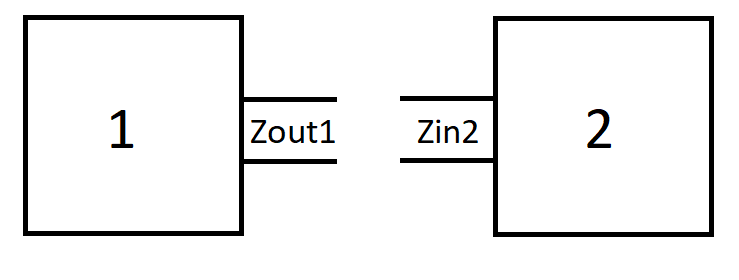
\includegraphics[width=0.3\linewidth]{matching}
	\label{fig:matching}
\end{figure}
\noindent
Q: What should be the relation between $Z_{out1}$ and $Z_{in2}$, so the impedances are "matched"?
\\
\\
A: The one of the numbers should be equal to complex conjugate of tother one, as presented in the equation below.
\begin{align*}
Z_{out1}\, &= \, {Z_{in2}}^*
\end{align*}
\\
The complex conjugate ($Z^*$) of given complex number $Z$ is defined in the following way:
\begin{align*}
Z &= x + j\cdot y \\
Z^* &= x - j\cdot y \\
\end{align*}
\section{Conclusions}
The introductory tasks covered basic, but essential aspects of microwave engineering. Expressing the ratio of powers or intensities in decibels is a common way to present these dependencies and matching impedances in the circuits is a common step in electrical equipment design,
\newpage
\chapter{Basics of Microwave Engineering}
\subsubsection{Problem statement}
Waveguides and transmission lines are both elements designed to be interconnects between receivers and transmitters of the EM waves (to be more precise -- in range of radio frequencies and microwaves). Despite having similar role, there are essential differences among their properties.

\begin{figure}[h]
	\centering
	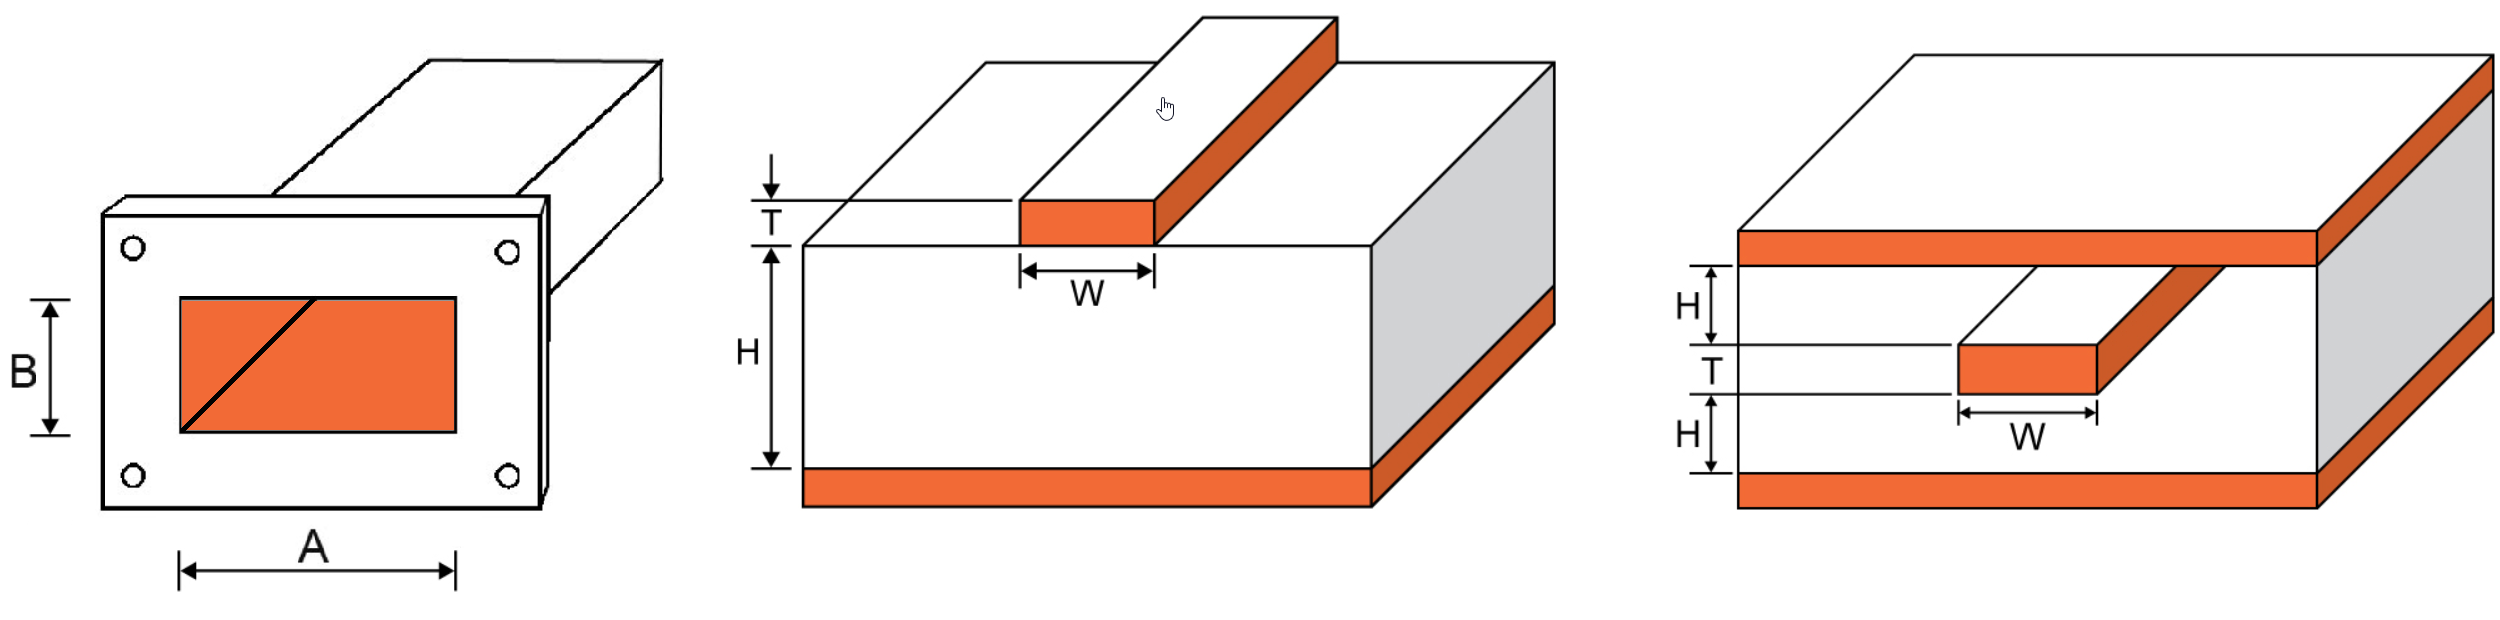
\includegraphics[width=0.8\linewidth]{technology}
	\caption{From left: waveguide, microstrip and stripline} (source: https://www.allaboutcircuits.com)
	\label{fig:technology}
\end{figure}

	
%\subsubsection{Waveguides review \footnote{Waveguide Primer -- Introduction, article in resource \cite{microwave}.}}

\subsubsection{Waveguides review }
The waveguide is manufactured out of one conductor (in opposite to printed lines, what will be cleared in next paragraph). It is said, that waveguide has certain advantages over the printed lines
%\footnote{Waveguide Primer -- Introduction \cite{microwave}.}
%\footnote{Ibidem.}
-- due to its shielding, it can provide the isolation between adjacent signals. In addition, it is capable to transmit high peak powers, while having negligible losses in range of microwave frequencies.\\
It is also worth mentioning, that all kind of waveguide components are available (circulators, isolators, attenuators, loads, mixers, amplifiers).
\\
On the other hand, there still remain the disadvantages such as small manufactured volumes coming with high prices of waveguides materials (copper and silver). Also the dimensions and weight of waveguide are significant. Because of above--mentioned single conductor, the waveguide cannot provide a transverse-electromagnetic mode of transmission.

\subsubsection{Printed lines review}
%\subsubsection{Printed lines review \footnote{Transmission lines -- Microstrip and Stripline, article in resource \cite{microwave}.}}
Transmission lines used in printed circuits boards manufacturing are microstrips and striplines.\\
The stripline is a conductor placed between a dielectric pair of ground planes ("sandwiched"). It is a TEM (Transverse Electro--Magnetic) transmission line, what means it is non--dispersive. It is one of stripline's advantage over the microstrips. Also, the isolation between adjacent traces can be achieved.\\
One of the disadvantages of stripline is its complexity in fabrication, what also makes it more expensive than microstrip. The second one is a result of the second ground plane. The strip widths shall be narrower for a given impedance and board thickness than microstrips. 
An example to illustrate, for replacing N mils thick microstrips, the stripline should be 4N mils thick.
\\
\\
The microstrip transmission lines is a conductive strip of certain dimensions (width and thickness) with the wider ground plane. They are separated by a dielectric layer called "substrate" (also characterized by another thickness dimensions). \\According to the "Microwave Encyclopedia", microstrips are the most popular transmission lines especially for MIMICs (Monolithic Microwave Integrated Circuits).
Its advantage over stripline is that all active components can be mounted on top of the boards. However, for filtering, they may be required to provide external shielding of the circuit. In addition to disadvantages, the microstrip circuits can radiate and are dispersive (signals of different frequencies travel with different speeds). The TEM mode is not supported.

\subsubsection{Summary}
As the three families of microwave components were introduced, it is essential to distinguish and sum--up their main features.\\
The waveguides are able to transmit high peak powers with very low losses in microwaves frequencies. Unfortunately, they are expensive and heavy equipment.
The striplines (conductor sandwiched between dielectric) are non--dispersive transmission lines supported TEM modes. They are more expensive than microstrip and more complex in fabrication.
The microstrips are at the moment very commonly used because of the ease of fabrication and usage. Unfortunately, they do not support TEM modes, often require external shielding and the circuit radiation has to be taken into consideration during the design process.

\newpage
\chapter{Microstrip vs stripline -- loss calculation using PCAAD}
\subsubsection{Problem statement}
During the class, there were given sets of parameters such as laminate and paths thickness, frequency, dielectric constant and impedance. The goal of the following task was to calculate total loss given in [dB/cm].\\
\\
The results are presented below in the tabular form.
\begin{figure}[h]
	\centering
	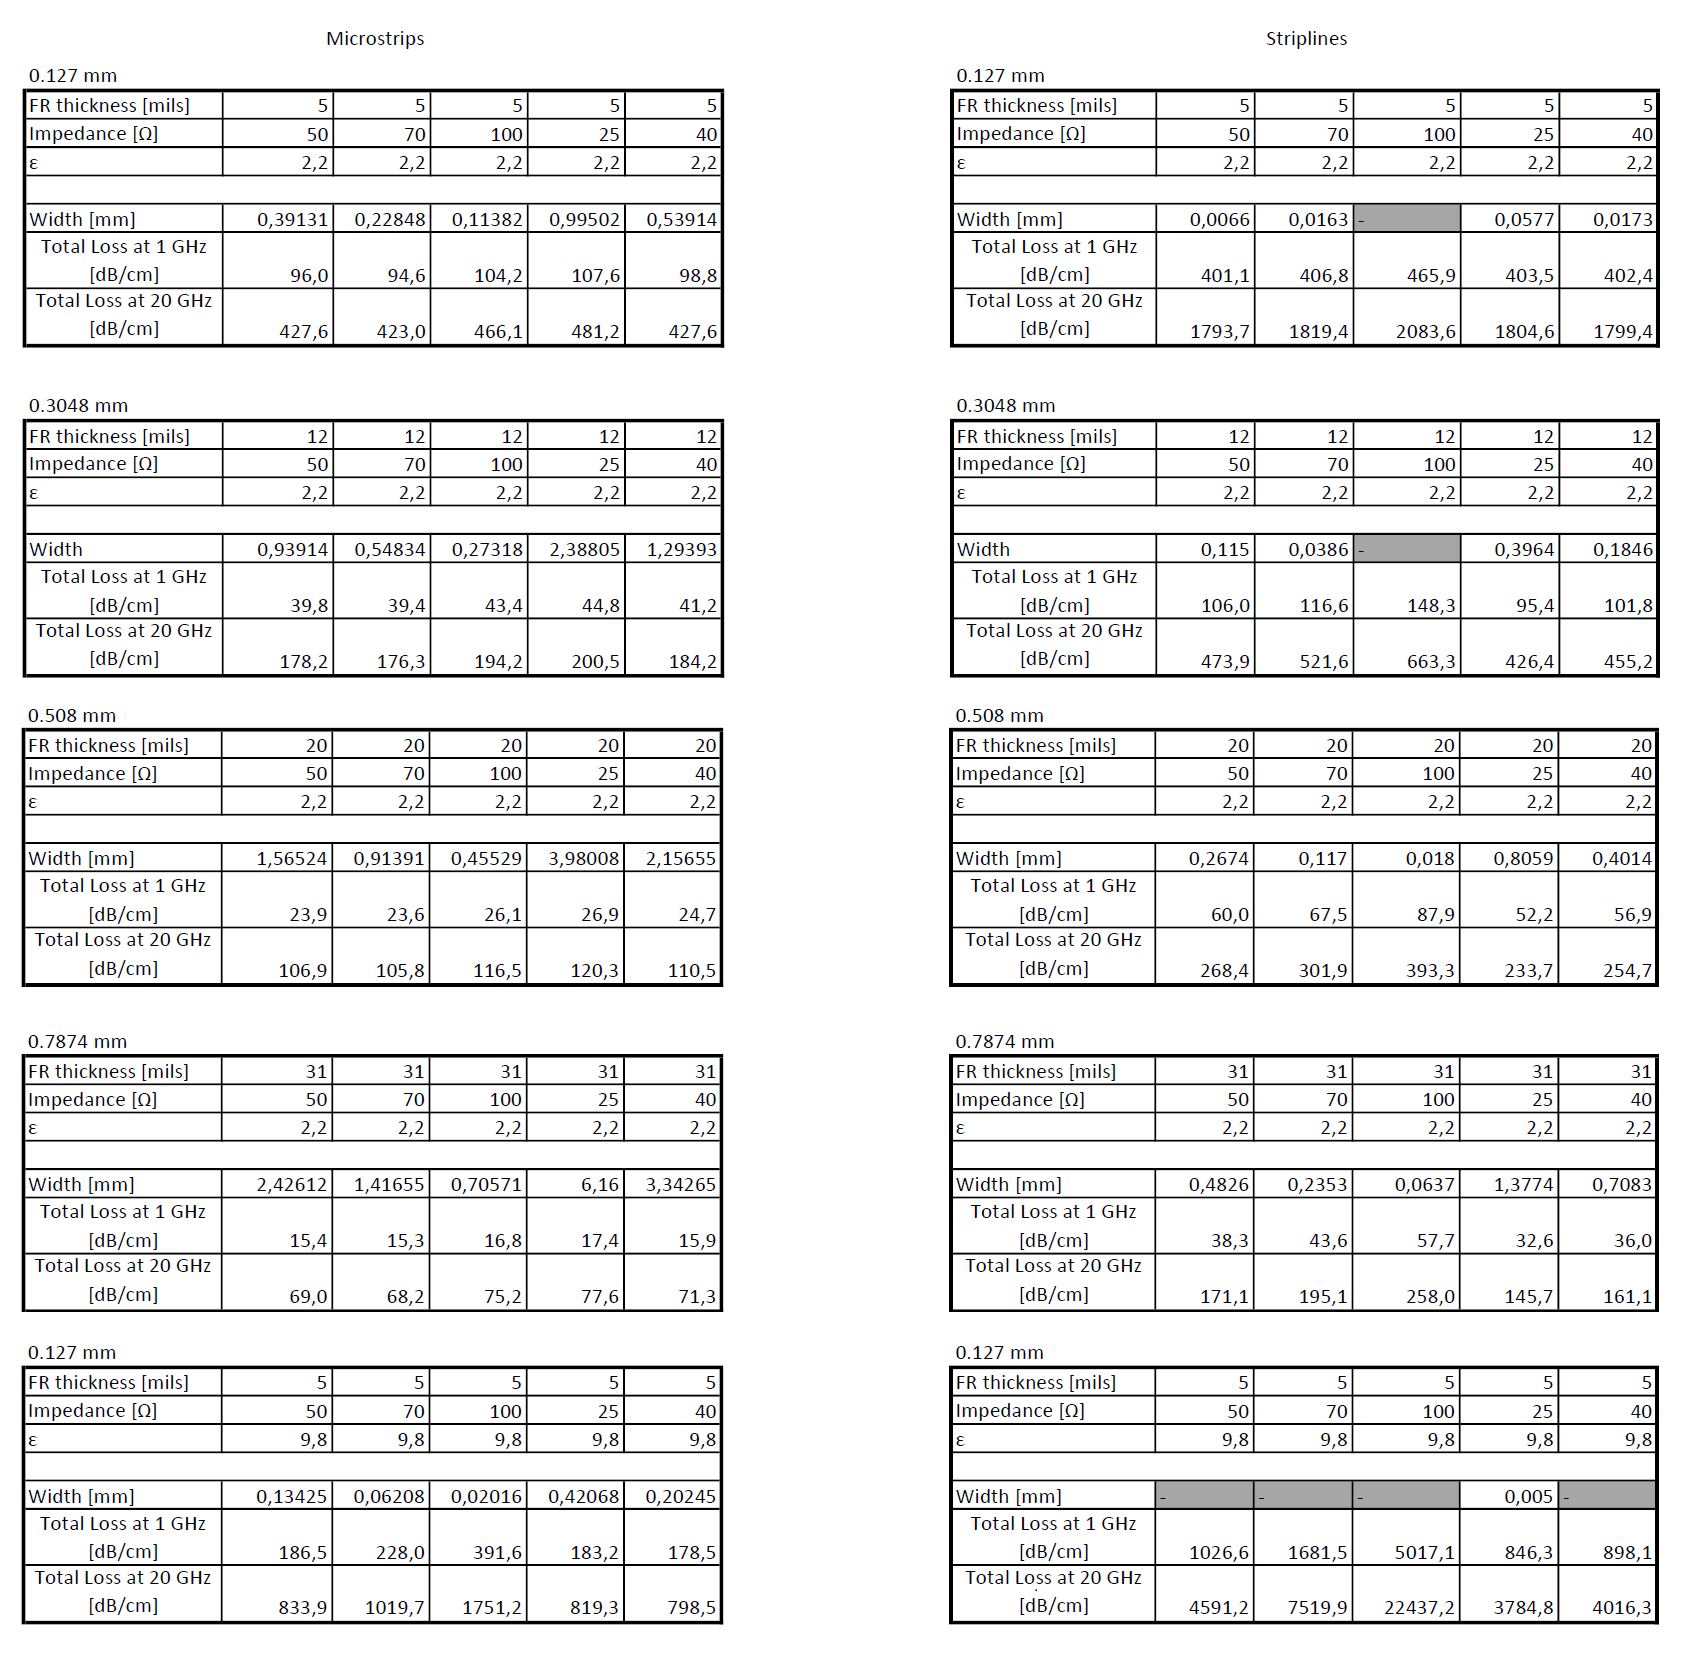
\includegraphics[width=1\linewidth]{microm1}
	\label{fig:microm1}
\end{figure}

\newpage
\begin{figure}[h]
	\centering
	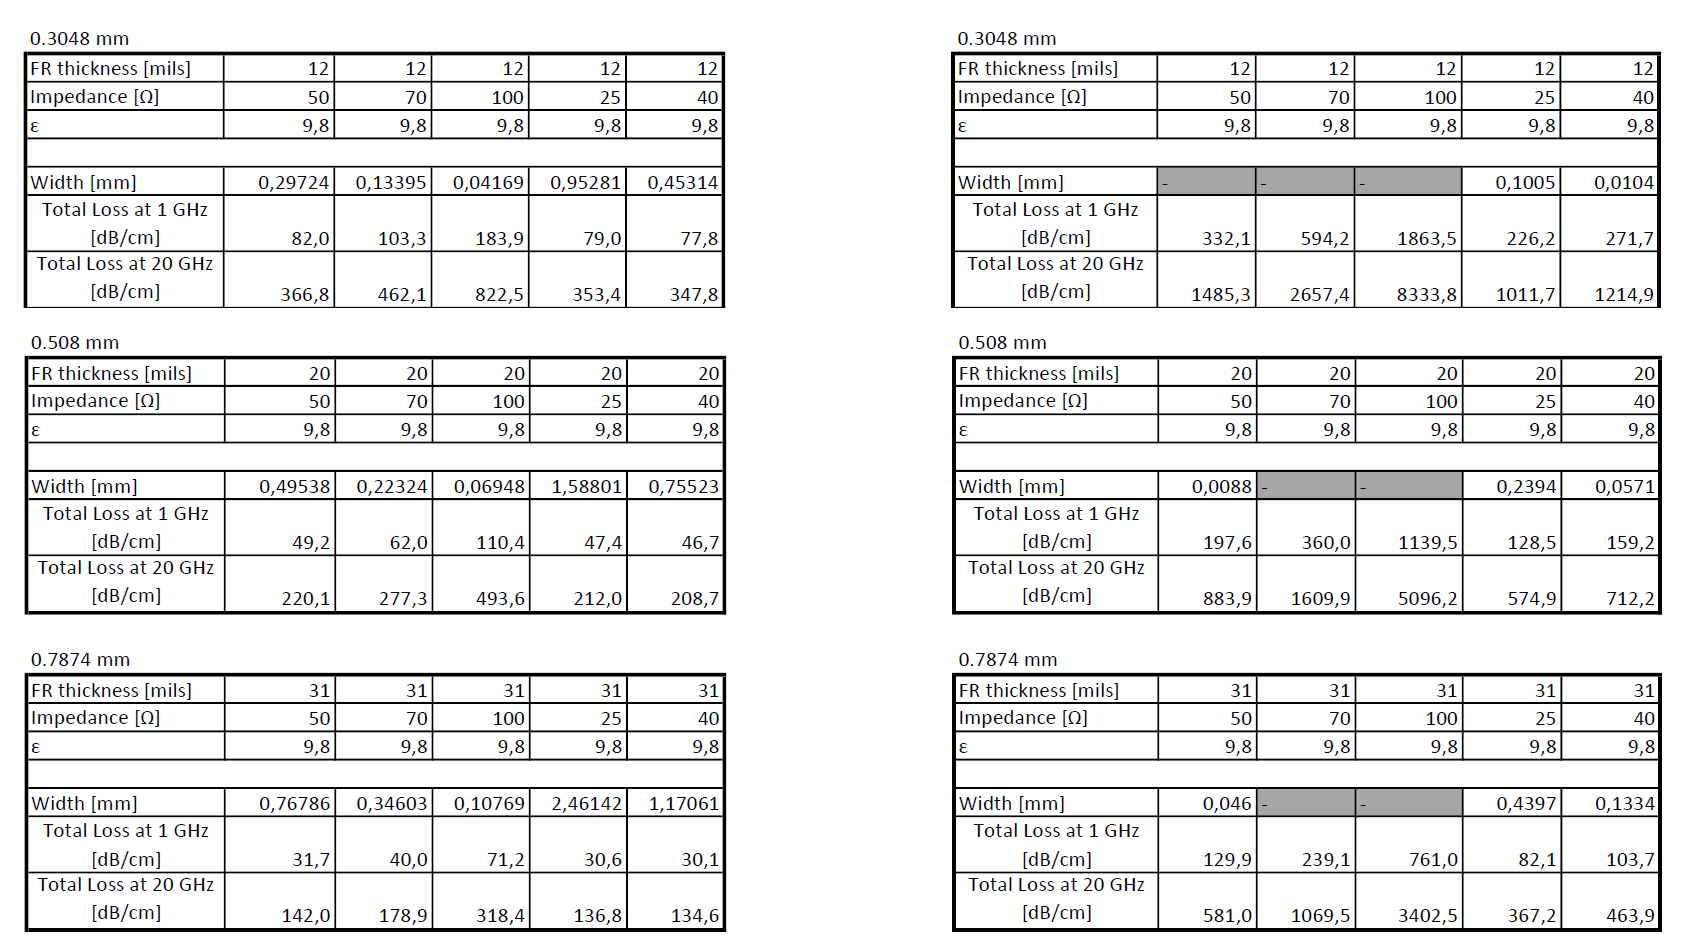
\includegraphics[width=1\linewidth]{microm2}
	\label{fig:microm2}
\end{figure}
\noindent
Some calculations (cells marked with gray color) were plain wrong either due to obtaining negative values of width or recevining \textbf{Nan} result (not a number).\\
Professor's piece of advice during the lab was to compare quasi--static analysis with full--wave. In some cases the results improved, however still there remain few unresolved.\\
\\
That lead to a very important conclusion -- the software for simulation has its limitations and it's much appreciated to use different tools (PCAAD, MicrowaveStudio, $\mu$Wave Wizard etc.).\\
\\
The assignment's second part was to compare the obtained results to the losses of waveguides:
\begin{figure}[h]
	\centering
	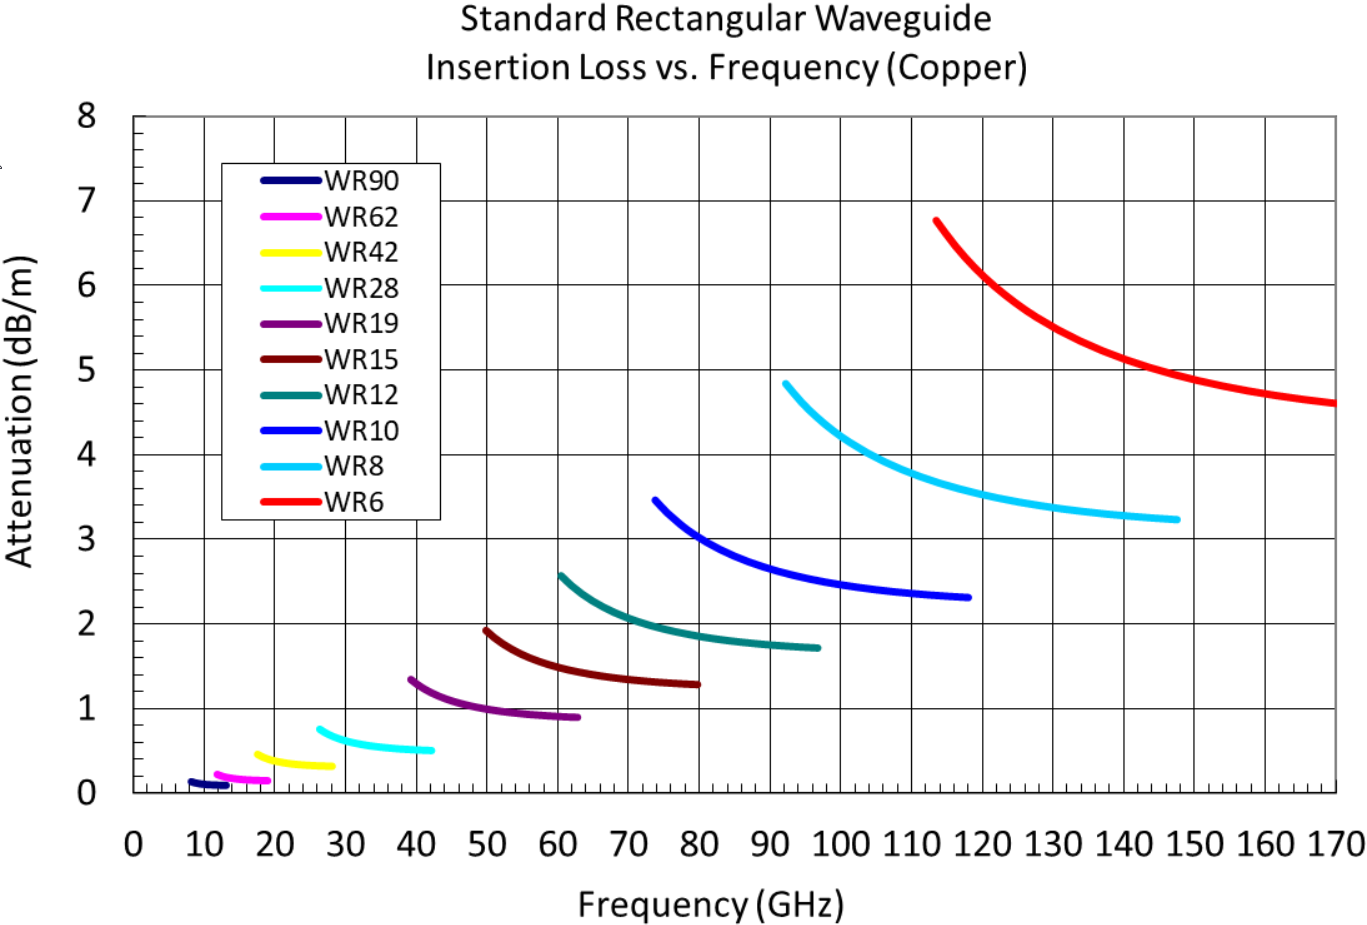
\includegraphics[width=0.6\linewidth]{waveguides}
	\label{fig:waveguides}
\end{figure}

\noindent
As it can be read from the plot -- waveguides offer much lower losses (and the Y--axis scale is in dB per METER).\\
The highest loses are presented for waveguide WR6, which is around \textbf{7 dB/m = 0.07 dB/cm}.
In terms of total losses, the microstrips and striplines cannot compete with the waveguides. 
\newpage

\chapter{Impedance transformation}
\subsubsection{Problem statement}
\begin{figure}[h]
	\centering
	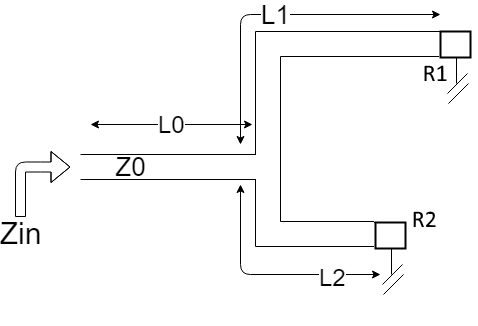
\includegraphics[width=0.7\linewidth]{impedance}
	\label{fig:impedance}
\end{figure}
\noindent
The presented above model was given to calculate the impedance transformation.
The data was defined in the following way:\\
R1 [0, 50, 70] $\Omega$,\\
R2 [0, 25, 50, 70]$\Omega$,\\
L0 $<$5, 200$>$mm with 25mm step,\\
L1 [13, 42, 72]mm\\
L2 [25, 42, 93]mm\\
\\
$f_0$ = 5 GHz\\
$\epsilon _r$ = 2.3,  tan$\delta$ = 0.001, laminate\_thickness = 0.508mm, copper = 18$\mu$
\\
\\
By utilizing the presented during classes equations, the impedance was calculated.\\
\begin{align*}
Z' &= \frac{Z_1 ' Z_2 '}{Z_1 ' + Z_2 '}\\
\\
Z_{in} &= Z_0 \frac{Z_L + jZ_0tan(\beta L)}{Z_0 + jZ_Ltan(\beta L)}
\end{align*}

\noindent
With the given data almost 1000 results were obtained (there was dedicated software script prepared in the Python language to calculate the impedance and automatically save the results as Excel file).
\\
\\
To maintain the clean view in the report, the results will be presented as the plots.
\begin{figure}[!h]
	\centering
	\subfloat[L1 == 13mm, L2 == 25mm, R1 == 0 Ohm]{{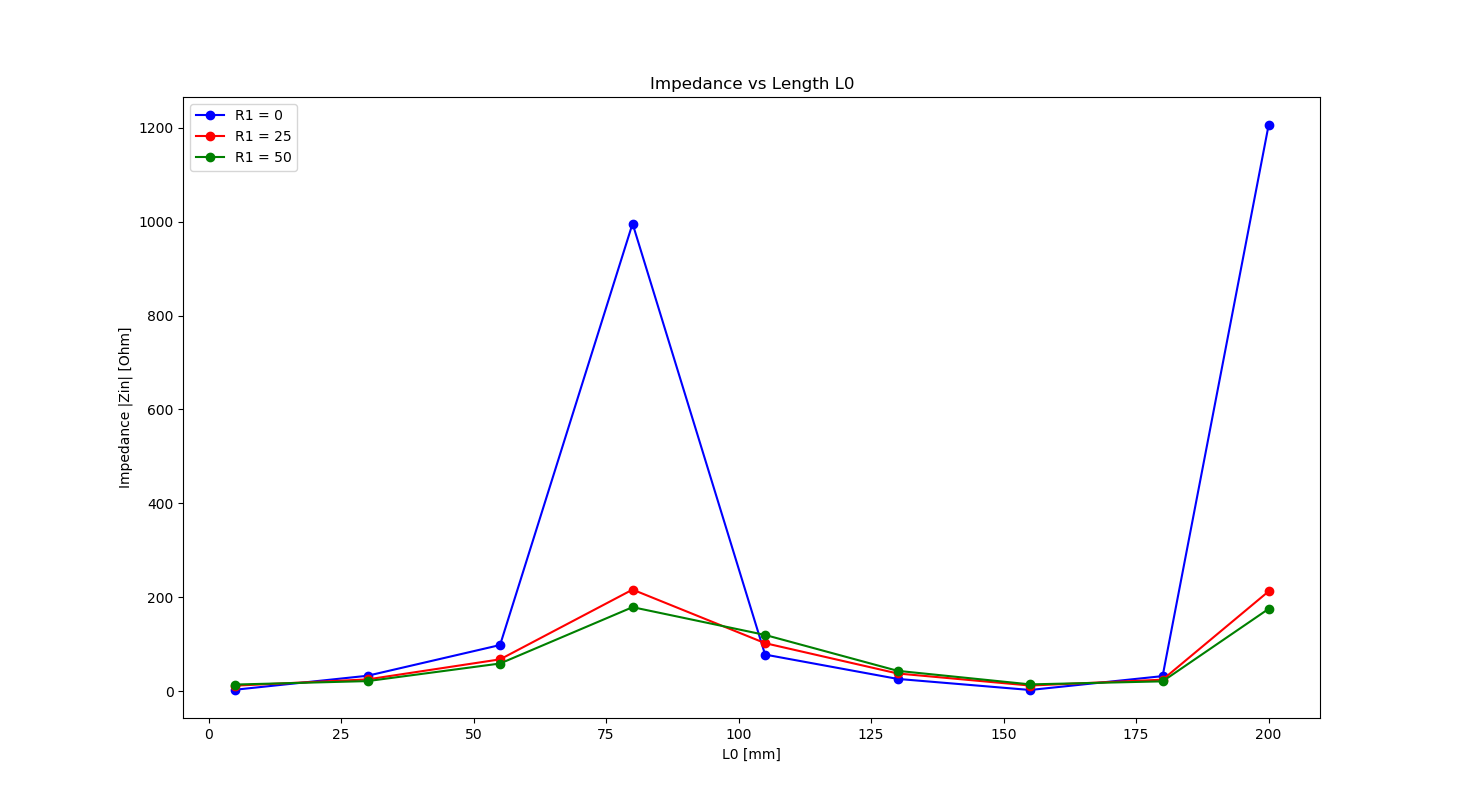
\includegraphics[width=0.5\linewidth]{Figure_4} }}%
	\subfloat[L2 == 13mm, L1 == 25mm, R2 == 0 Ohm]{{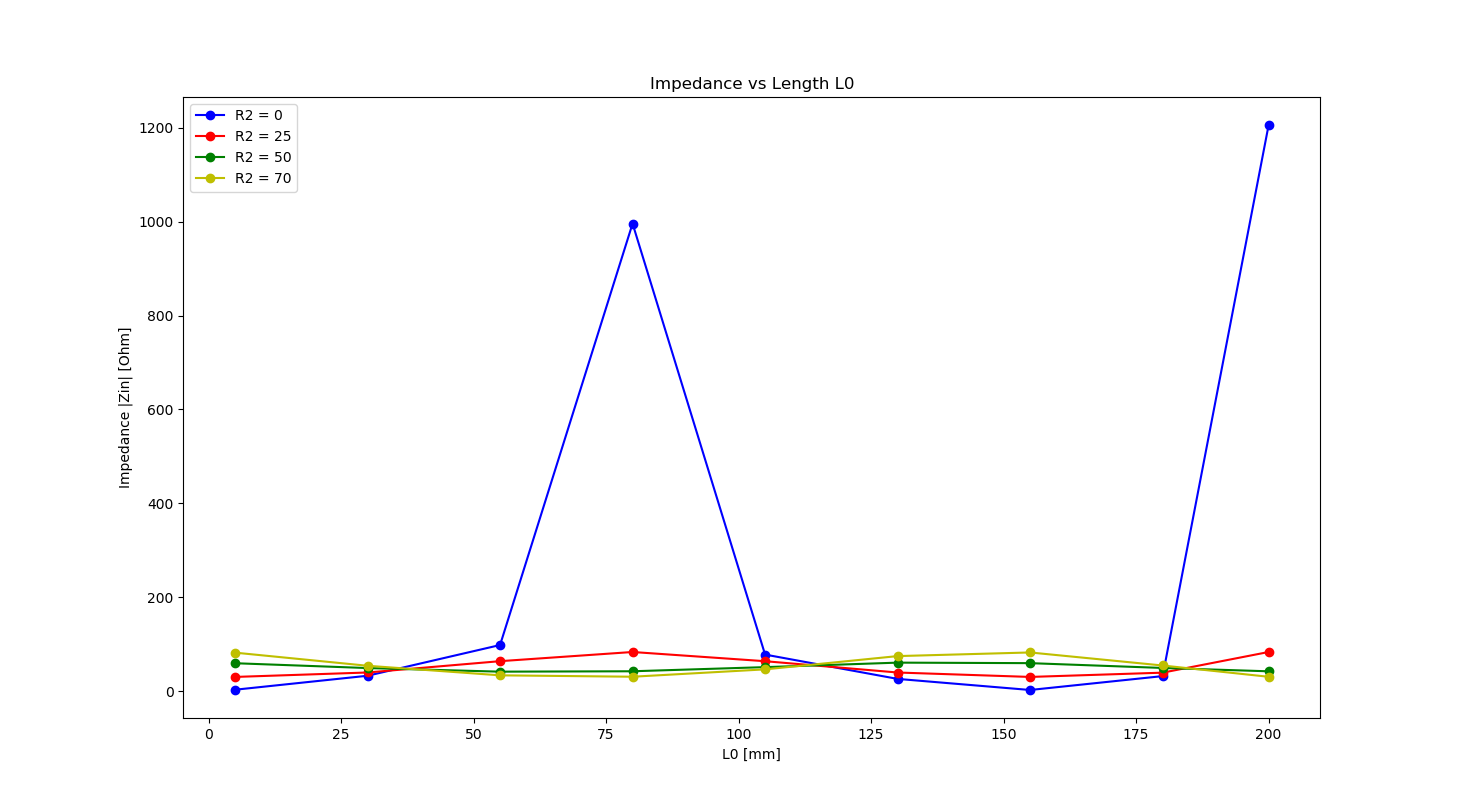
\includegraphics[width=0.5\linewidth]{Figure_5} }}%	
	\caption{Relation between L0 and magnitude of impedance Zin}
	\label{fig:figure1}
	\centering
	\vspace{30pt}
	\subfloat[L0 == 30mm, L1 == 13mm, L2 == 25mm, Ohm]{{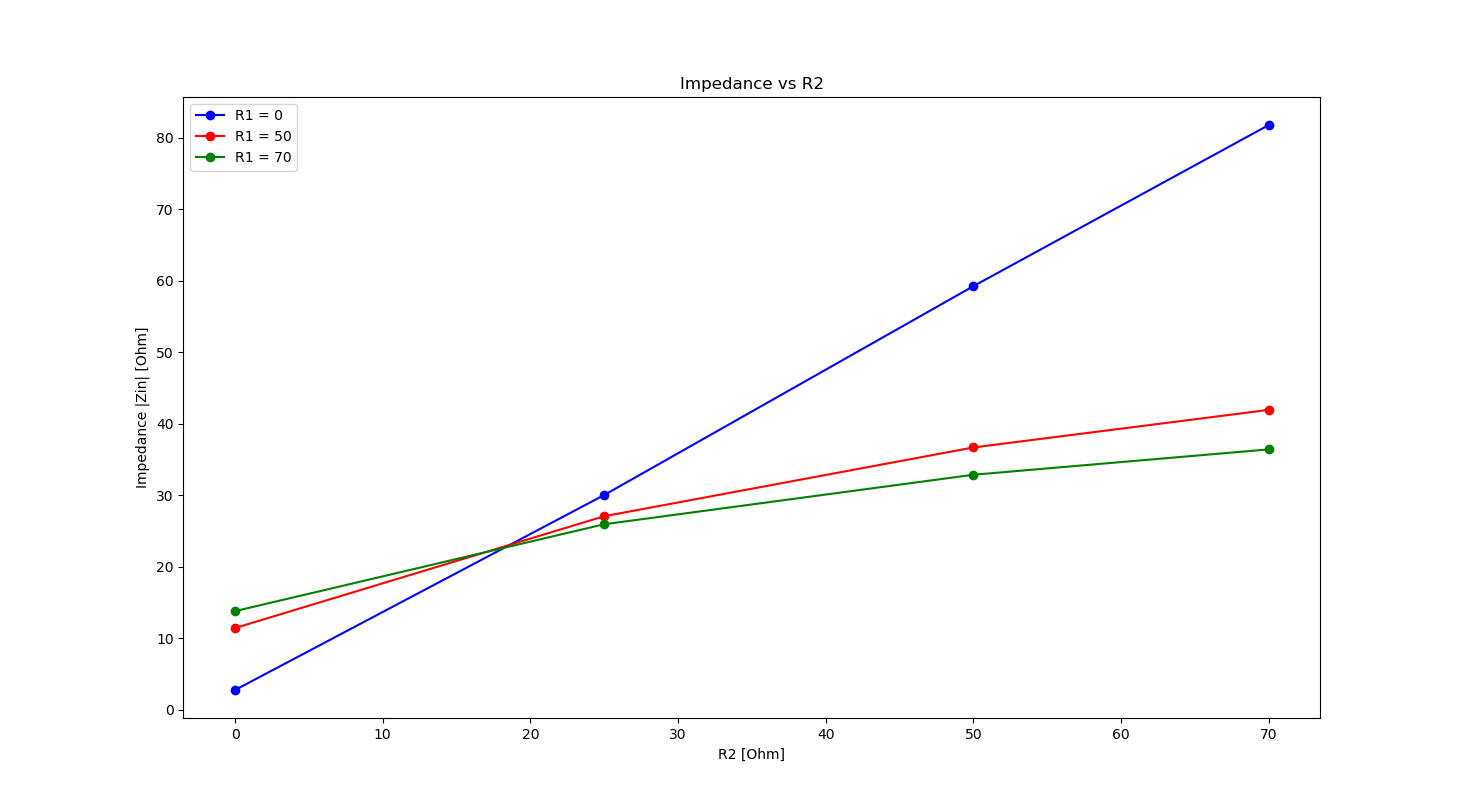
\includegraphics[width=0.7\linewidth]{Figure_1} }}%
	\caption{Relation between R2 (x-axis), R1 (curves family) and magnitude of impedance Zin}
		\vspace{30pt}
	\centering
	\subfloat[L0 == 30mm, L2 == 25mm]{{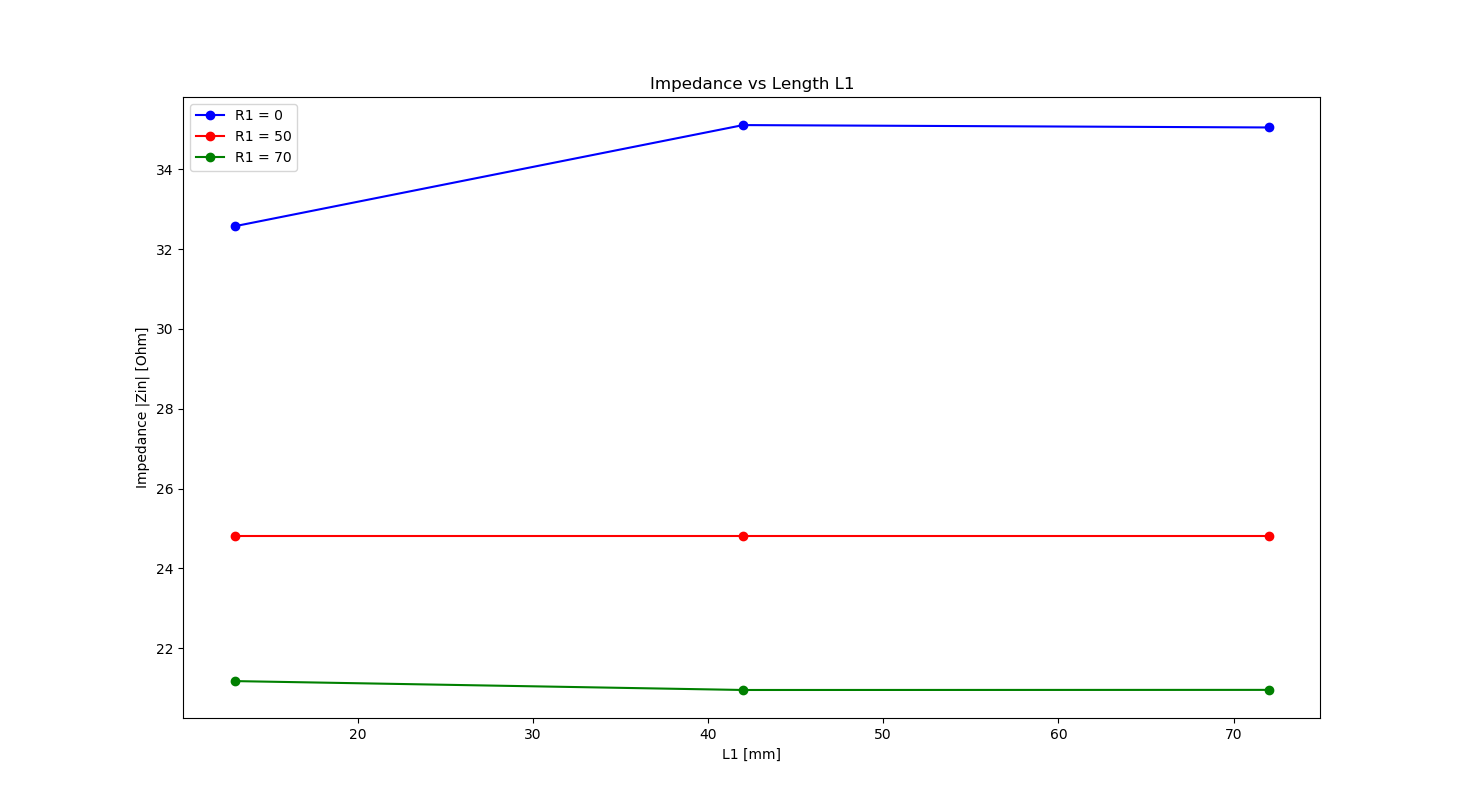
\includegraphics[width=0.5\linewidth]{Figure_2} }}%
	\subfloat[L0 = 30mm, L1 == 13mm]{{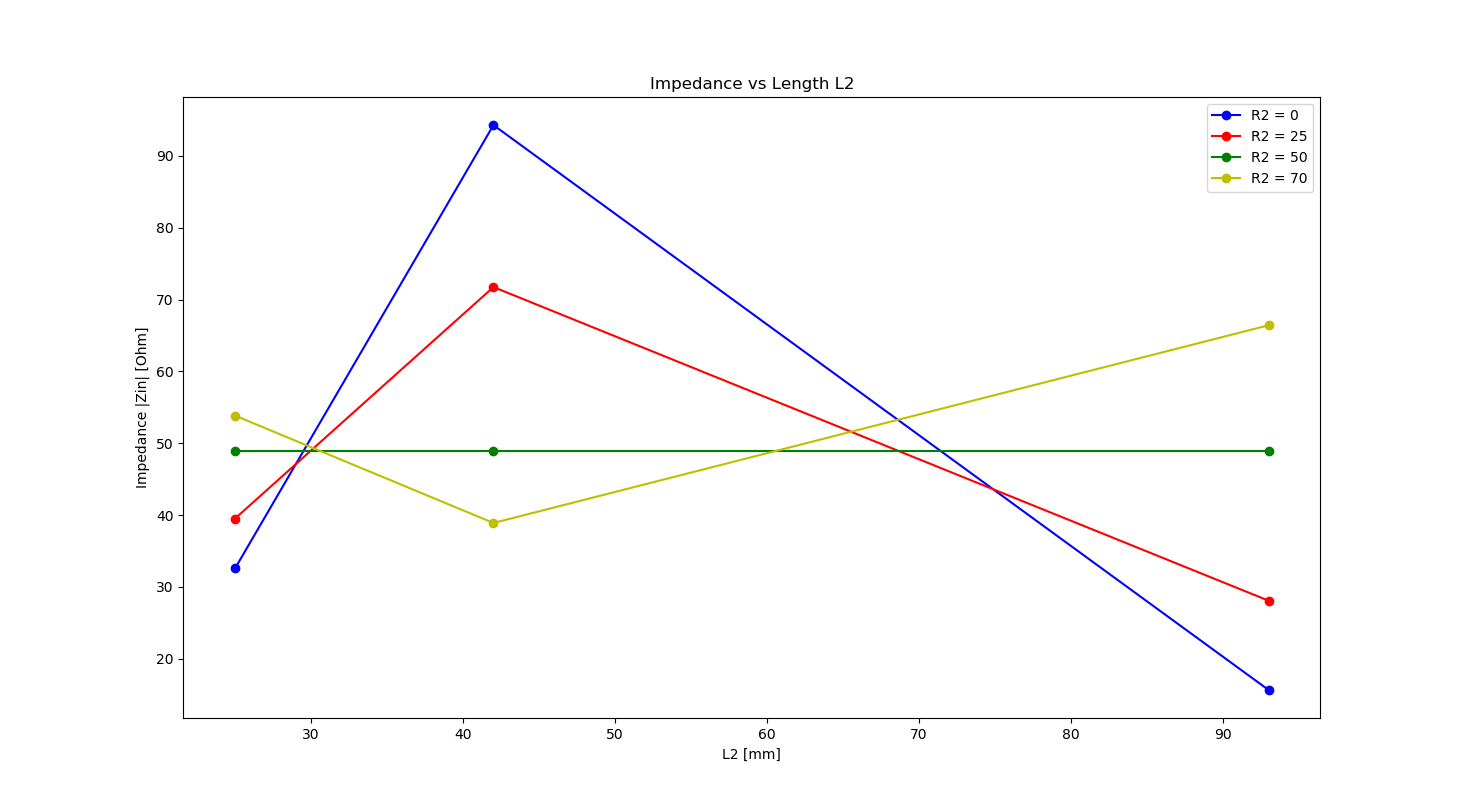
\includegraphics[width=0.5\linewidth]{Figure_3} }}%
	\caption{Relation between lengths L1, L2 and magnitude of impedance Zin}
	\label{fig:figure1}
\end{figure}
\\

\newpage

\chapter{HMC778LP6CE -- fractional--n PLL with integrated VCO}
\subsubsection{Problem statement}
\begin{figure}[!h]
	\centering
	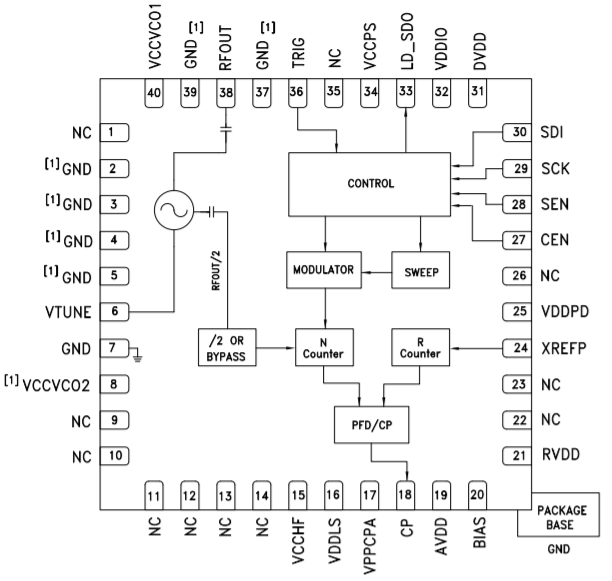
\includegraphics[width=0.3\linewidth]{pll}
	\label{fig:pll}
\end{figure}
\noindent
\subsubsection{Circuit information}
The HMC778LP6CE is a fully functioned Fractional-N Phase-Locked-Loop (PLL) Frequency Synthesizer with an
integrated Voltage Controlled Oscillator (VCO). \\
The official datasheet is describing the input reference frequency range to be DC to 350 MHz. The manufacturer claims that it provide very good phase noise performance over temperature,\\
shock and process. The HMC778LP6CE offers frequency sweep and modulation features, external
triggering, double-buffering, exact frequency control, phase modulation.\\ \\ The HMC778LP6CE is packaged
in a leadless QFN 6 x 6 mm surface mount package.

\subsubsection{PLL operation}
The assignment was to prepare a short summary of principles of PLLs operation of the HMC778 circuit and to describe the difference in operation between integer and fractional PLLs.
\\
The basic application of PLL integrated circuit such as HMC778 is to form a control loop to multiply low frequency source to a higher frequency.\\
The phase detector and charge--pump drive the tuning signal of VCO (voltage controlled oscillator) to bring the phases (phases of both reference signal and tuning signal) at the detector input into alignment.\\
\\If the loop succeeds, then the phase detector inputs (reference and DIV at the diagram) are at the same frequency. 
As the frequency of DIV = $f_{VCO} / N$, then its equality means that control loop forced the frequency of VCO to be N $\cdot f_{PD}$.
\begin{figure}[!h]
	\centering
	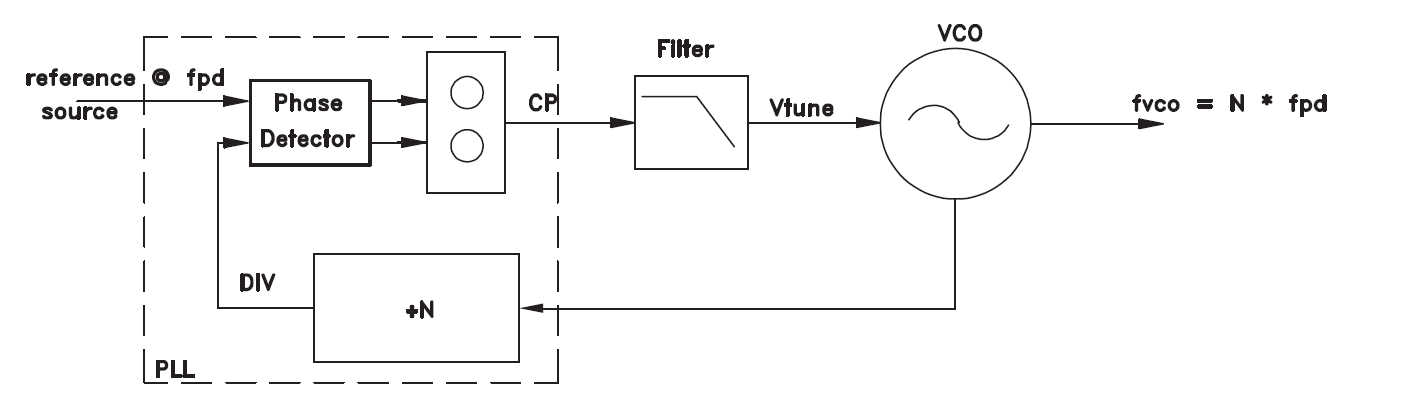
\includegraphics[width=0.7\linewidth]{pll3}
	\label{fig:pll3}
\end{figure}
The difference between integer and fractional PLL is that the fractional can bring N value at fractional level (1.6, 2.4, 3.7) while the integer can do it only with discrete value of N (2, 4, 10, 13 etc.).
\newpage
\subsubsection{Designing PCB for HMC778}
\begin{figure}[!h]
	\centering
	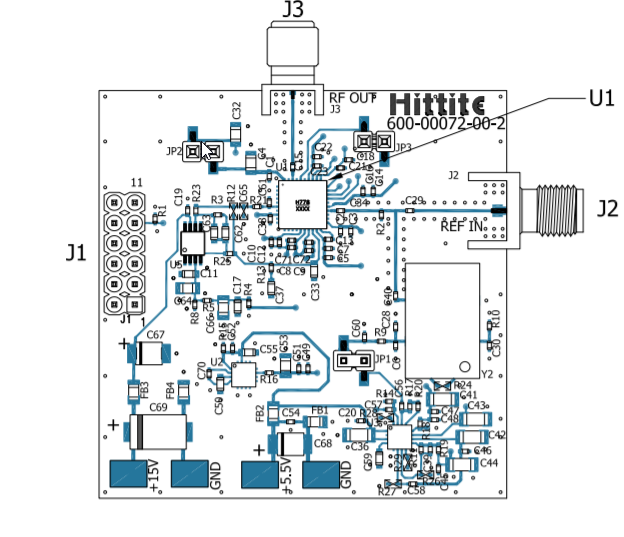
\includegraphics[width=0.3\linewidth]{pll2}
	\label{fig:pll2}
\end{figure}
Guidelines to design a PCB board:
\begin{itemize}
	\item The circuit board used in the application should use RF circuit design techniques. 
	\item Signal lines should have
	50 Ohm impedance while the package ground leads and exposed paddle should be connected directly
	to the ground plane. 
	\item A sufficient number of via holes should be used to connect the
	top and bottom ground planes.
\end{itemize}

\chapter{Free--space path losses}
\subsubsection{Problem statement}
During the laboratory, we discussed the aspect of free--space losses and started the evaluation according to the distance.\\
This task was to finish the calculations we started and prepared the comparison in the tabular form.

\begin{table}[h]
	\centering
	\caption{The comparison of free--space losses in relation to used frequency and distance between transmitter and receiver}
	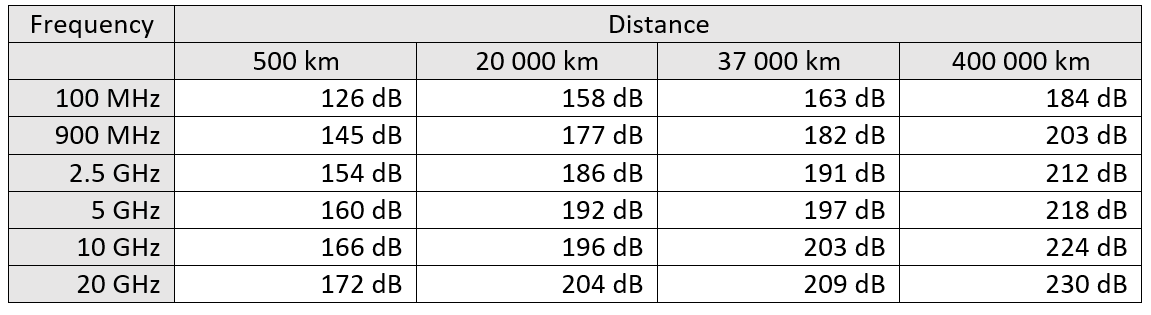
\includegraphics[width=0.9\linewidth]{freespace}
	\label{fig:freespace}
\end{table}
\noindent
The table observation leads to a clear conclusion -- the free--space losses are increasing with the longer distance and when using high frequencies.
\newpage
\chapter{Microwave low--noise amplifier operating at C--band}
\subsubsection{Problem statement}
The C--band is a portion of the electromagnetic spectrum in the microwave range of frequencies ranging from 4.0 to 8.0 GHz (according to IEEE designation).\\
To fulfill the given assignment, the packed low noise amplifier manufactured by Qorvo was chosen. It is \textbf{TGA2611-SM} model, operating at frequency range 2.0 - 6.0 GHz, so its range of operation covers C--band.
\\
It is said, that the product is designed to commercial and military radars or communication.\\
Its noise figure is estimated to be 1.0 dB.
\begin{figure}[h]
	\centering
	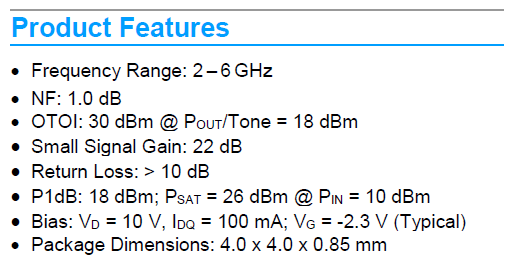
\includegraphics[width=0.3\linewidth]{chip}
	\caption{Basic features of selected amplifier.}
	\label{fig:chip}
\end{figure}

\noindent
The *.s2p file describing the scattering matrix of the plot was obtained from the Qorvo site. In the Ansoft Designer there was prepared a report:
\begin{figure}[h]
	\centering
	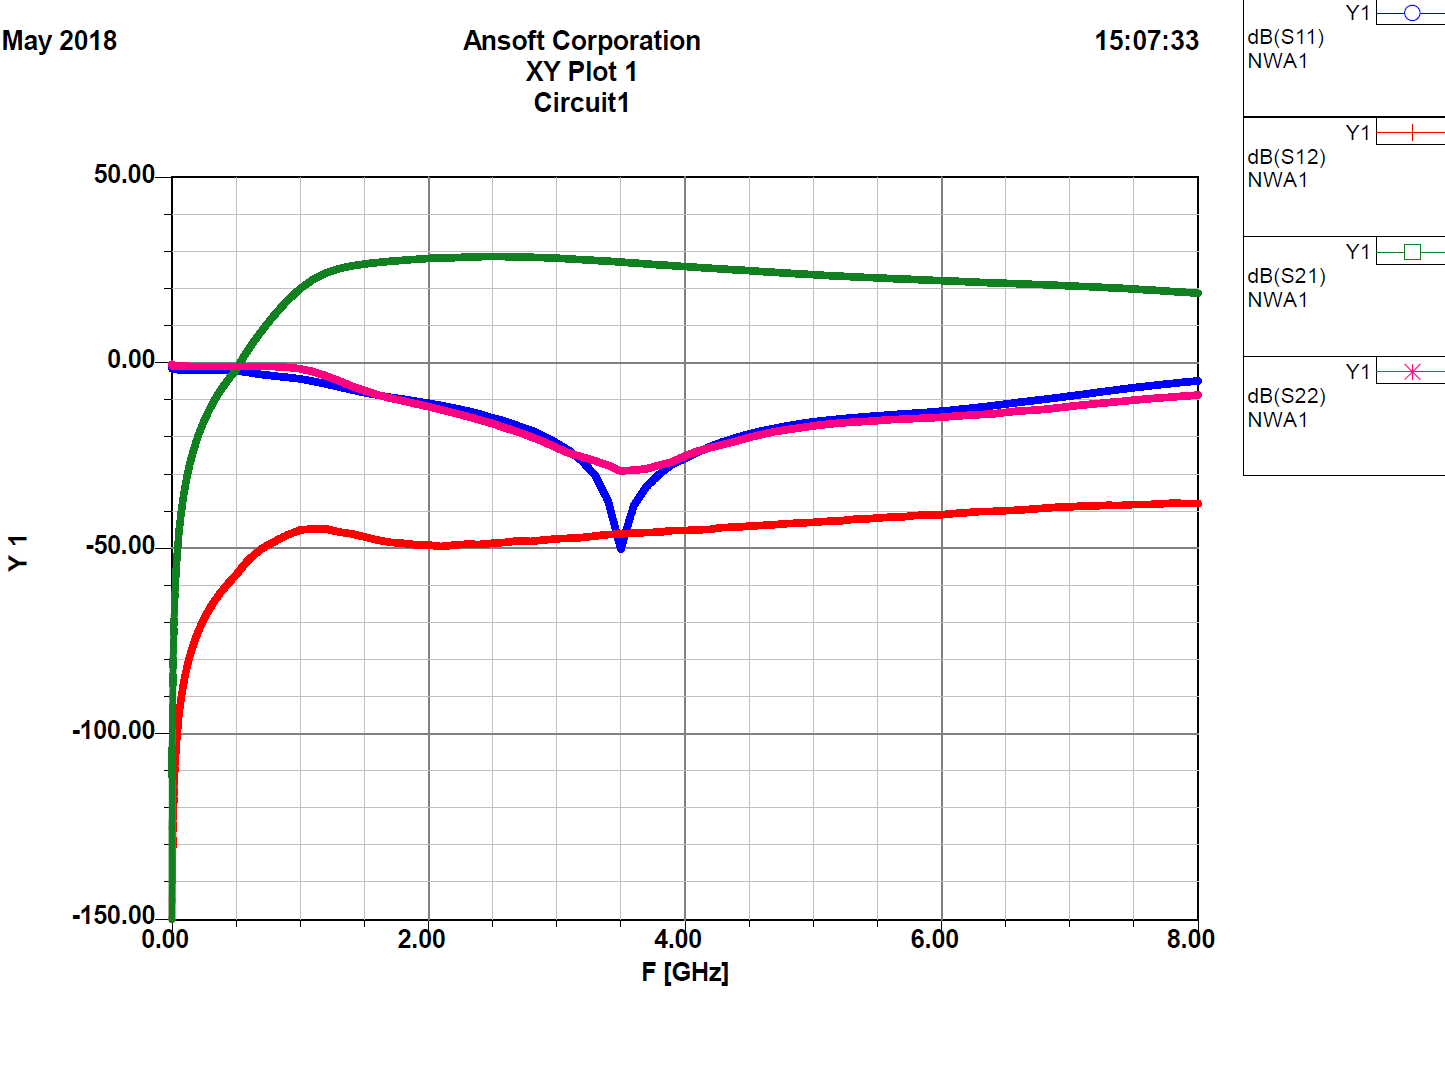
\includegraphics[width=0.7\linewidth]{chip-plot}
	\caption{Plot of the scattering matrix.}
	\label{fig:chip-plot}
\end{figure}

The Scattering matrix describes the following aspects of the N--port element:
\begin{itemize}
\item S11 input return loss  (blue plot)
\item S12 reverse gain       (red plot)
\item S21 small signal gain  (green plot)
\item S22 output return loss (pink plot)
\end{itemize}

\subsection*{Noise Figure}
The plot below presents the noise figure of the selected amplifier.
\begin{figure}[h]
	\centering
	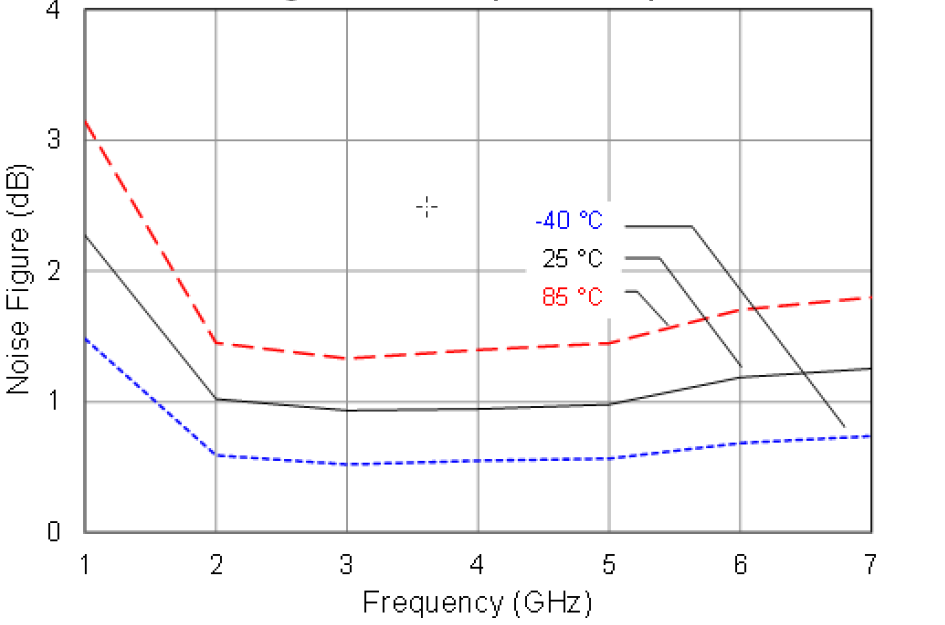
\includegraphics[width=0.6\linewidth]{noise}
	\caption{Noise figure vs frequency (at different temperatures).}
	\label{fig:noise}
\end{figure}

\subsection*{}
Despite advertised 1dB noise figure in the operating range (reminder: 2 -- 6 GHz), when approaching the upper limit of 6 GHz the NF increases. However, the change is very insignificant (more or less it is 1.25 dB).\\
Of course also the temperature is important, but also at 85 $^\circ$C
the NF in operating range is around 1.75 dB.
\begin{thebibliography}{9}
\bibitem{microwave} Online Microwave Encyclopedia, http://microwave101.com,  (27.02.2018)
\end{thebibliography}
	
\end{document}